\pattern{Layered}
\begin{summary}
    A layered architecture style divides components into layers with specific
    functions. For each unique project, there is no specified number of layers
    that it must possess and developers decide on the number of layers
    depending on the needs of the project. This architecture is best suited for
    microservices, and systems without much business logic to complicate
    relationships between layers.  This is because each layer is only required
    to fulfill its own responsibilities without taking on the responsibilities
    of the other layers for the sake of organization. Over the years, it has
    become the most popular style due to its simplicity, ease of development,
    and organization.  
\end{summary}

\comparison{\begin{itemize}
        \item Testability: Components can be mocked or stubbed since they
            belong to specific layers of the architecture. Due to this, it is
            relatively easy to test functionality of isolated functionalities.
            For example, a presentation component can be mocked to focus on
            testing a business component, or the business layer can be mocked
            to test certain aspects of the presentation layer.

        \item Maintainability: Layers are created to separate the concerns of
            the components. As an example, business logic should only be
            contained in the business layer. Because of this, if there are
            changes to one layer, other layers’ components should not be
            affected, making layers easy to update and maintain for future
            changes.

        \item Ease of development for teams: Since this pattern is very well
            known and simple to understand, it also provides teams with ease of
            development. Different people are usually given tasks specific to
            their domain of knowledge, so it makes sense for each person to
            focus on their tasks without having to understand all parts of the
            application. As an example, a person who works on the presentation
            layer does not need to know how data is stored in the database
            layer. Likewise, a person that works on the database layer does not
            need to understand how the presentation layer is implemented. Thus
            the architecture supports the non-functional requirement of
            complexity.

        \item Cohesion: If each layer is well defined and only contains
            functions that are related to the needs of that layer, the layer
            has high cohesion. For example, the database layer should only have
            components which deal with writing, querying, and generally
            managing the data.

        \item Coupling: Each layer is considered to be either open or closed.
            Requests can bypass open layers, while if the layer is closed the
            request must go through that layer. There should be clear
            documentation or communication of which are open and closed, and
            the reason for their implementation. Depending on their
            architecture, layers can provide low coupling. However, a layered
            architecture can have high coupling, which is a disadvantage, if
            software developers or architects do not follow best practices.

\end{itemize}
}{\begin{itemize}
        \item Low Scalability: Due to the nature of layered architecture being
            very simple, it is difficult to use its principles on larger and
            more complex projects. This is due to the architecture being
            monolithic in nature, and further organization and complexity is
            difficult to implement without abstracting from the layered
            principle. For example, it is possible to further abstract each
            layer adding complexity but it is difficult to keep the simple
            layered architecture principles. Therefore, since the architecture
            offers little support and guidelines for expanding to meet the
            requirements of larger and more complex projects the non functional
            property of scalability is low.

        \item Inefficiencies: As perceived from the diagrams thus far, a
            potential request may have to go through multiple layers to fulfill
            a request. Although this can be somewhat alleviated with open and
            closed layers, the architecture as a whole suffers from general
            inefficiency as requests need to often go through multiple layers
            instead of one source. Difficult to Deploy: In cases where layers
            or components (a common pitfall using the architecture
            historically) within the layer are highly coupled, it creates a
            scenario where layers or components highly depend on each other.
            Then, it becomes that changing one component needs several other
            components to be affected and thus rebuilt, which takes time. Thus,
            it is often not efficient for highly coupled layers to be used in
            things like a continuous deployment pipeline.
            
        \item Low Agility: Also due to the potential coupling, the pattern
            itself may have low agility which is a non functional property
            which measures how the architecture responds to quick continuous
            changes. Although some features can be isolated in this pattern, if
            components or layers are highly coupled, changing a component may
            cause the developer to need to make changes in other components and
            layers if they depend on each other. Since coupling between
            components within layers is a common pitfall using this
            architecture, it generally does not meet the non functional
            property of agility.
\end{itemize}}

\begin{nfps}
\item[Description] See above.
\end{nfps}

\begin{center}
    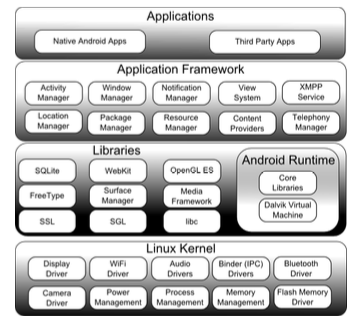
\includegraphics[width=0.4\textwidth]{./layered}
    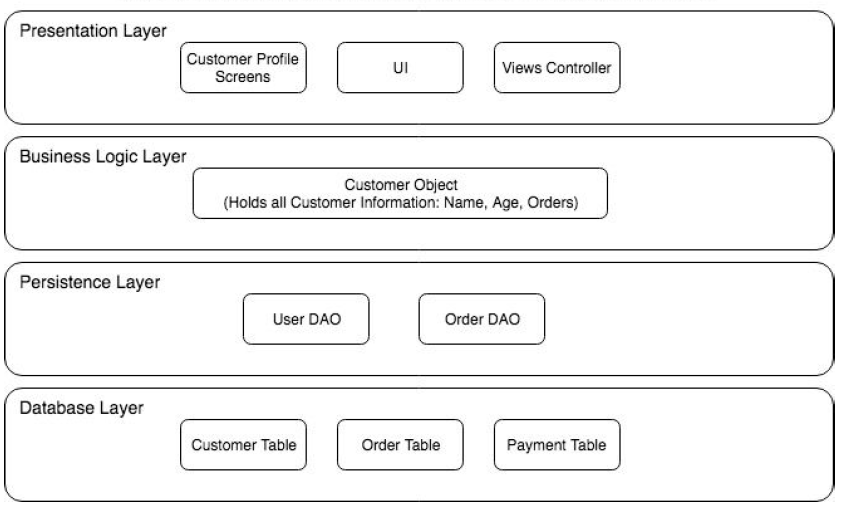
\includegraphics[width=0.4\textwidth]{./layered2}
\end{center}
